\documentclass{report}
\usepackage[francais ]{babel}
\usepackage[utf8]{inputenc}
\usepackage[T1]{fontenc}
\usepackage{graphicx}
\usepackage{float}
\usepackage{hyperref}
\usepackage{array}
\title{Mini Games}

\author{M. \textsc{Friedli}, A. \textsc{Gillioz}, J. \textsc{Guerne}\\
He-Arc Ingénierie\\
2000 Neuchatel}
\date{\today{}}
\begin{document}
\maketitle{}

\begin{abstract}
La HES d'été permet aux étudiants de deuxième année d'étude dans le domaine de l'informatique
la possibilité de travailler sur un projet libre dans le but d'approfondir leurs connaissances.

Ce rapport décrit, explique les choix d'implémentations pris dans la réalisation de notre
projet Mini Games.

Une planification des tâches ainsi qu'une spécification du travaille ont été réalisés dans le but
d'organiser au mieux le temps à disposition.
\end{abstract}
\tableofcontents

\chapter{Introduction}
Mini Games est une application offrant la possibilité de jouer à des minis jeux très classique tel
que le morpion ou la bataille navale en réseau et en multi-platforme. C'est à dire que deux personnes
l'une sur son téléphone android et l'autre sur son ordinateur auront la possibilité de se défier à une partie de jeu en ligne.
Deux grands outils ont été utilisés pour faciliter l'implémentation de ce projet, il sagit du framework Libgdx, qui a servit à
deployer le même programme sur différentes platforme, et de la libraire kryonet, qui a elle facilitée les échanges réseau.

Les jeux listés dans le cahier des charges sont les suivants :
\begin{itemize}
	\item Morpion
	\item Bataille navale
	\item (Bonus : Jeu de dame)
\end{itemize}
L'objectif principal de ce projet n'est pas de développer des jeux compliqués et très
développé mais plutôt de se concenter sur le multi-plateforme et le réseau.

\chapter{Planification}

Nous avons réparti le travail selon les affinités, compétences et disponibilités de chacun.
\par
\begin{itemize}
	\item Gestion client - serveur : Jonathan Guerne
	\item Morpions : Jonathan Guerne
	\item Bataille navale : Anthony Gilloz
	\item User Interfaces : Jonathan Guerne et Marc Friedli
	\item Test : Jonathan Guerne, Anthony Gilloz et Marc Friedli
	\item Rapport : Jonathan Guerne, Anthony Gilloz et Marc Friedli
	\item Relecture : Marc Friedli
\end{itemize}
\par
Nous avons ensuite déterminer les principales tâches à réaliser et leur avons donné un ordre de priorité (Figure \ref{planif}).

\begin{figure}[H]
	\centering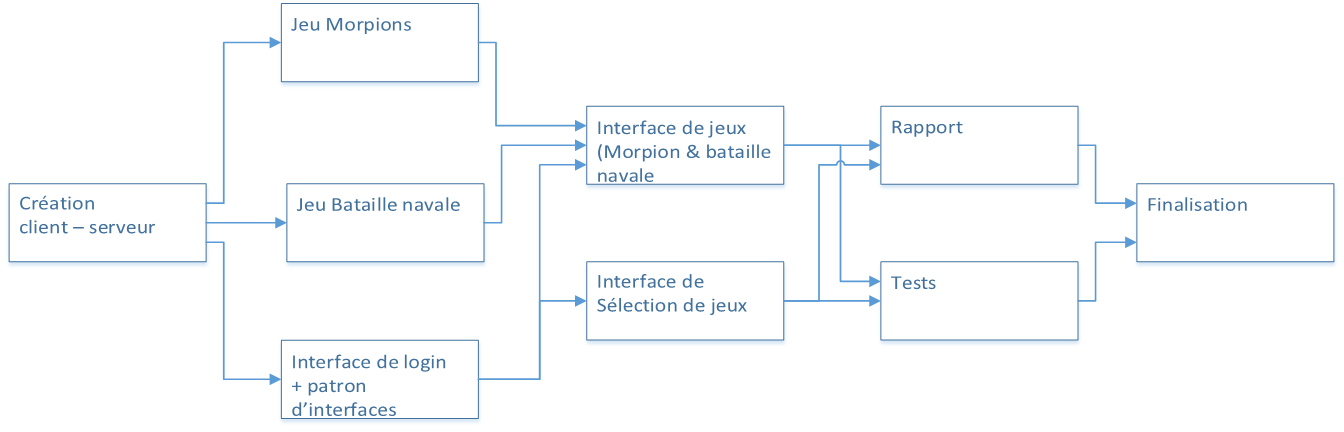
\includegraphics[width=15cm]{Planif}
	\caption{Ordre de réalisation des tâches}
	\label{planif}
\end{figure}

\chapter{Conventions de nommages}
Le code a été écrit en respectant la convention camelCase pour les variables et
les méthodes. Le camelCase consiste à commencer les noms par des minuscules et si
le nom est une composition de plusieurs mots utiliser une majuscule comme séparateur.
Les classes respectent la convention PascalCase qui reprend les mêmes conventions que
le camelCase excepté le fait que les noms commencent par des majuscules.
Les verbes sont privilégiés lors du nommage de méthode par soucis de clarté.
L’utilisation de l’anglais plutôt que le français a été préféré.

\chapter{LibGDX}
\begin{figure}[H]
	\centering
\includegraphics[width=9cm]{libgdx}
	\caption{Logo de LibGDX}
\end{figure}
Dès le lancemment du projet, nous nous sommes orienté vers libGDX qui est un
framework Java gratuit et open source permettant la conception de jeux vidéo.
Nous avons fait le choix de travailler avec ce framework en particulier, car
nous avions découvert son existence quelque temps auparavant et, en apprenant à le connaître,
nous avons découvert à quel point il facilite le déploiement multi-platforme.
LibGDX nous a permis de gagner en temps précieux au niveau de l’implémentation
puisqu’il propose nativement des fonctionnalités comme la gestion de stages ou
de cameras qui sinon aurait dû être créés à la main.
Étant un framework connu et grandement utilisé, il est simple de trouver des
renseignements ou de l’aide concernant sa façon de fonctionner. Nous n’avions
aucune expérience dans son utilisation pourtant il ne nous a fallu que très peu
 de temps avant de commencer à d’obtenir de bons résultats.

\chapter{Kryonet}
\begin{figure}[H]
	\centering
\includegraphics[width=9cm]{kryonet}
	\caption{Logo de Kryonet}
\end{figure}
Ayant travaillé cette année sur des échanges réseau en Java sans utiliser de libraire externe nous avons pu réaliser que la tâche était fastidieuse, c'est donc naturellement que nous
nous sommes tourné vers Kryonet qui est une librairie open source permettant de faciliter la communication entre différents clients. Un des points essentiel du projet était de pouvoir
garentir que LibGDX et Kryonet pouvaient cohabiter, après quelques tests et recherches nous avons pu réaliser que c'était bel et bien ée cas ( du moins pour le déploiment sur ordiateur et android).

\chapter{Architecture logicielle}
L'architecture logicielle détaille les choix qui ont été pris durant l'implémentation du projet.

Pour optimiser le codage et donc viser à obtenir un code K.I.S.S. (keep it simple and stupid) nous avons choisi de réfléchir sur la logique d'impplémentation
des classes à l'aide de différents diagramme avant de commencer le projet. Nous avons donc pu réfléchir
aux différents problèmes potentiel et aux différents moyens de rendre de code plus apte à être retravailler plus tard (ajout de fonctionnalités).

\section{Diagramme de classe}
Le diagramme de classe a été réalisé au début du projet dans le but de donner une direction au projet, il a ensuite été généré en fin de projet
dans le but de présenter de façon condensé tous les élémensts du projet (voir figure \ref{diagramme de classe client figure} et \ref{diagramme de classe serveur figure}).

\begin{figure}[H]
	\centering\includegraphics[width=15cm]{classdiagrammclient}
	\caption{Diagramme de classe du programme client}
  \label{diagramme de classe client figure}
\end{figure}

\begin{figure}[H]
	\centering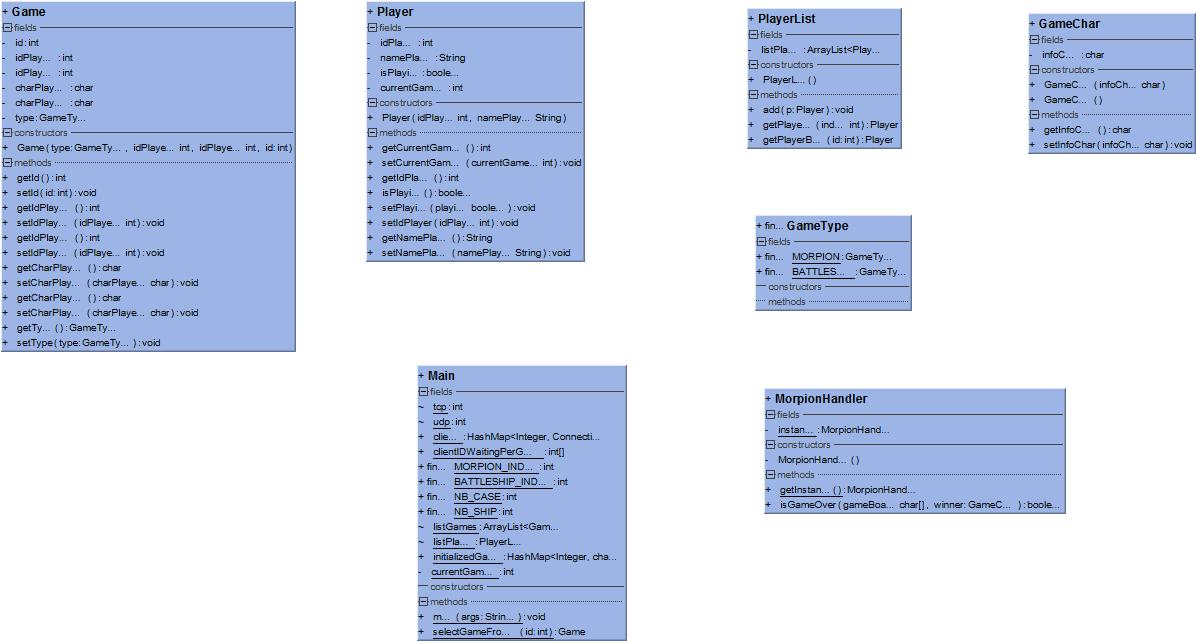
\includegraphics[width=15cm]{classdiagrammserver}
	\caption{Diagramme de classe du programme serveur}
  \label{diagramme de classe serveur figure}
\end{figure}

\chapter{Communication réseau}
Comme dit plus haut, le programme est une collection de minis jeux auxquels les clients auront la possibilités de jouer à
plusieurs. Le programme est décomposé en deux parties : la partie client et la partie serveur. La communication entre ces
deux parties est facilitée par l'utilisation de Kryonet une librairie Java open source conçu pour gérer les échanges réseau.

\begin{figure}[H]
	\centering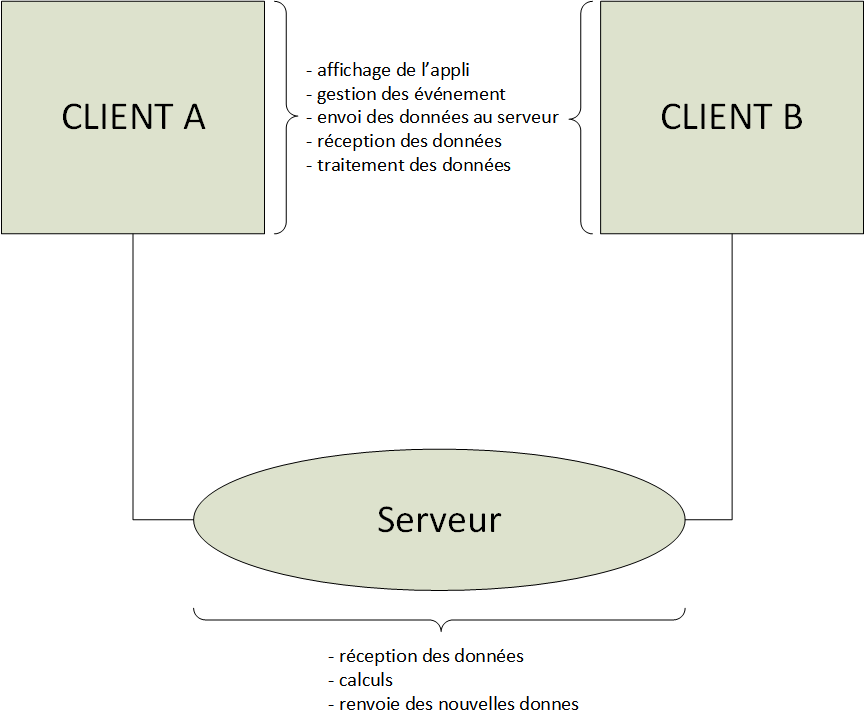
\includegraphics[width=10cm]{maquette_Base}
	\caption{Illistration de la communication entre les clients et le serveur}
\end{figure}


\section{Les packets}
Les données envoyées entre le client et le serveur transitent sous la forme de Packets, les packets sont des classes présentent
chez le client et chez le serveur enregistrer au lancement du service.

Pour un client, si une connexion à été établie, il lui est possible d'envoyer par
TCP ou UDP des Packets au serveur. Dans le cas complémentaire,
pour recevoir les différents Packets émmanent du serveur le client met en place
un listener qui va automatiquement gérer la réception des Packets et analyser leur contenu.
L'implémentaion du serveur est identique à la nuance près qu'elle laisse le choit
de la personne (de l'adresse) à qui sera envoyé le Packets. En effet toutes les infos, tous les Packets,
transitent par le serveur, c'est lui ensuite qui les traitent et les renvoient aux différents clients conscernés.

Pour que le serveur et le client puissent travailler avec les mêmes packets en plus de
possèder les mêmes classes ses classes doivent être enregistrées avec le bon identifiant auprès de
Kryonet. Les identifiants sont ici de simple integer.

\begin{tabular}{|l|c|}
\hline
 Identifiant du Packets & Domaine d'utilisation \\
\hline [0-999] & Login et configuration générale \\
\hline[1000-1999] & Packets liés au morpion \\
\hline[2000-2999] & Packets liés à la bataille navale \\
\hline
\end{tabular}

\section{Sécurité}
Pour empêcher des versions obselettes de se connecter au serveur un système de version a été mis en place.
Chaque Packets qui transite possède une version, le serveur peut tester si cette version est suffisamment
récente avant même d'analyser le contenu du Packet envoyé, si le Packet à une version trop vielle le serveur n'en fera rien.
En absence de réponse du serveur le joueur ne pourra donc pas se connecter.


\section{Initialisation de la connexion}
A l'ouverture du programme le client est invité à entrer une adresse de serveur
et un pseudo pour tenter ensuite de se connecter. Afin de faciliter l'entrée de l'adresse du serveur la fonction de
découverte des hôtes fournie par Kryonet a été utilisée, elle va fournir une
liste d'adresse qui seront ensuite présentées à l'utilisateur sous la forme d'une liste déroulante
si l'utilisateur sélectionne un élément de la liste l'adresse est automatiquement copié dans le champs de l'adresse du serveur.

Une fois que le serveur à reçu un Packet de login (une tentative de connexion a
été envoyée) le serveur stocke le nouveau joueur dans une liste, il comfirmera ensuite le
bon déroulement des opération au client en lui envoyant un Packet de confirmation.
Ce Packet de confirmation le client l'utilise comme signal pour changer d'écran
et afficher le menu de sélection des jeux.

\section{Communication en jeu}

Quand un joueur décide de lancer une nouvelle partie d'un jeu il transmet un Packet au serveur donnant comme information son ID et le jeu
auquel il shouaite jouer. Le serveur va, une fois le Packet reçu, verifier si quelqu'un est déjà en train d'attendre de démarrer un partie de ce jeu
ou non. Comme ce projet n'implémente que des jeux à deux joueurs la "salle d'attente" pour jouer à un jeu ne sera jamais composée de plus d'une personne,
ce joueur (ou plutôt son ID) est stocké dans un variable faisant office de salle d'attente du jeu désiré.

Quand un second joueur se connecte la pertie peu commencer ! le serveur prépare donc un Packet de création de partie contenant l'ID et le nom de tous les
joueurs de la partie, mais également le numéro (également appelé ID) de la partie en elle même (utile plus tard).

Tour à tour les joueurs envoient des informations aux serveurs propre au jeu auquel ils sont en train de jouer, le serveur va ensuite lui se charger de
tester si la partie est terminée ou non et enverra les bons Packets en conscéquence.

Quand une partie est finie un message s'affiche chez les joueurs leur idiquant s'ils ont gagné, perdu ou encore fait un match nul (morpion). Ils sont
ensuite invité à cliquer sur l'écran pour revenir à la sélection des minis jeux.

Si un joueur quitte la partie alors qu'elle n'est pas terminé le serveur en est informé. Il récupère ensuite les informations de la partie que
ce joueur était en train de faire et contact son adversaire pour lui signaler l'abandon de son adversaire.

\chapter{Minis jeux}
Dans ce chapitre seront présentés les différents minis jeux mis en place dans
ce projet aisni que leur implémentation.
Le serveur garde un historique des jeux sous la forme d'une liste d'objets
contenant les informations sur les différents joueurs opposés durant la partie.

\section{Morpion}
\label{Morpion}

\subsection{Description}
Le morpion est un jeu très simple dans lequel deux joueurs s'affronte sur un plateau de 3 x 3 cases. Chaque joueur possède des caractère (joueur 1 'x' et joueur 2 'o').
Tour à tour, ils vont devoir placer ces cartacères dans le plateau de jeu dans le but de faire une ligne horizontale,verticale ou encore diagonale.
Si la partie se finit sans qu'aucun joueur n'ai réussi à remplir une ligne/ une diagonale c'est un match nul.
\subsection{Implémentation}

Quand un joueur démarre une partie s'il ne trouve pas d'adversaire il est mis en attente. Un message lui signalant l'attente d'un
adversaire s'affiche sur l'écran, une fois le second joueur connecté l'écran de jeu s'affiche (figure \ref{attente_adversaire}).

\begin{figure}[H]
	\centering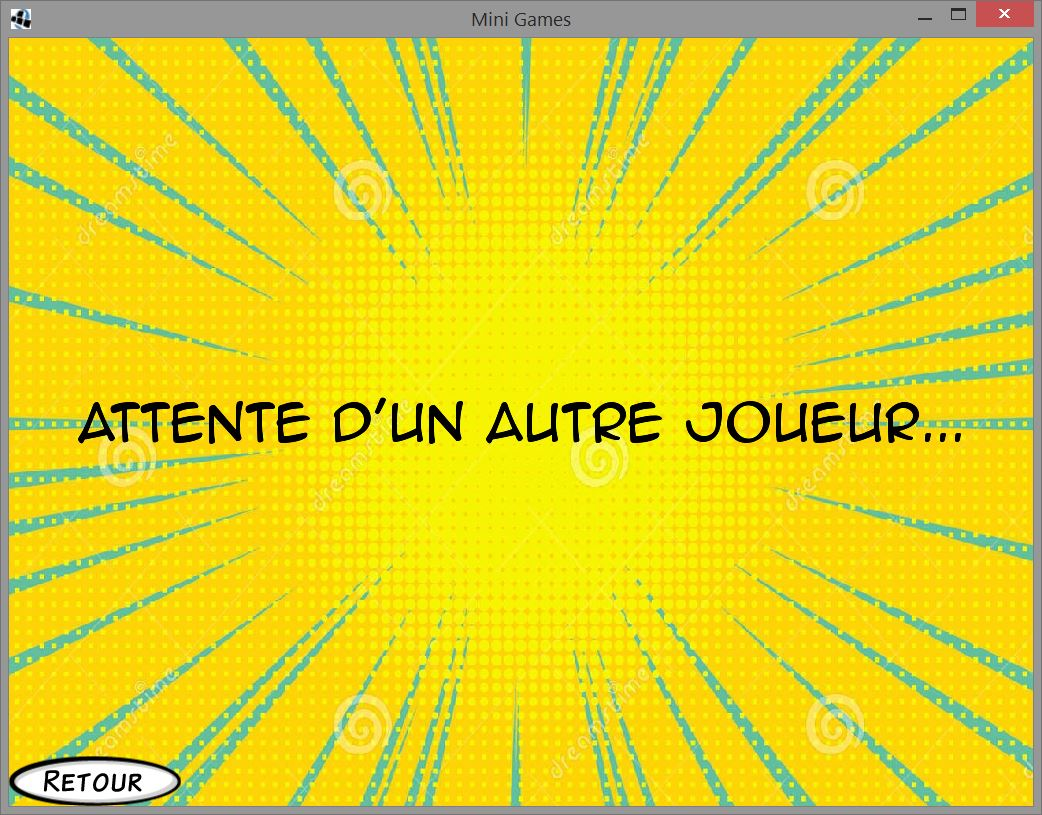
\includegraphics[width=9cm]{morpionwaiting}
	\caption{Attente d'un adversaire}
  \label{attente_adversaire}
\end{figure}

L'écran de jeu est composé en 2 parties : des informations sur la partie ainsi qu'un bouton "retour" se sithue en haut
de l'écran, tout le reste est occupé par le plateau de jeu (figure \ref{morpion_en_jeu}).

\begin{figure}[H]
	\centering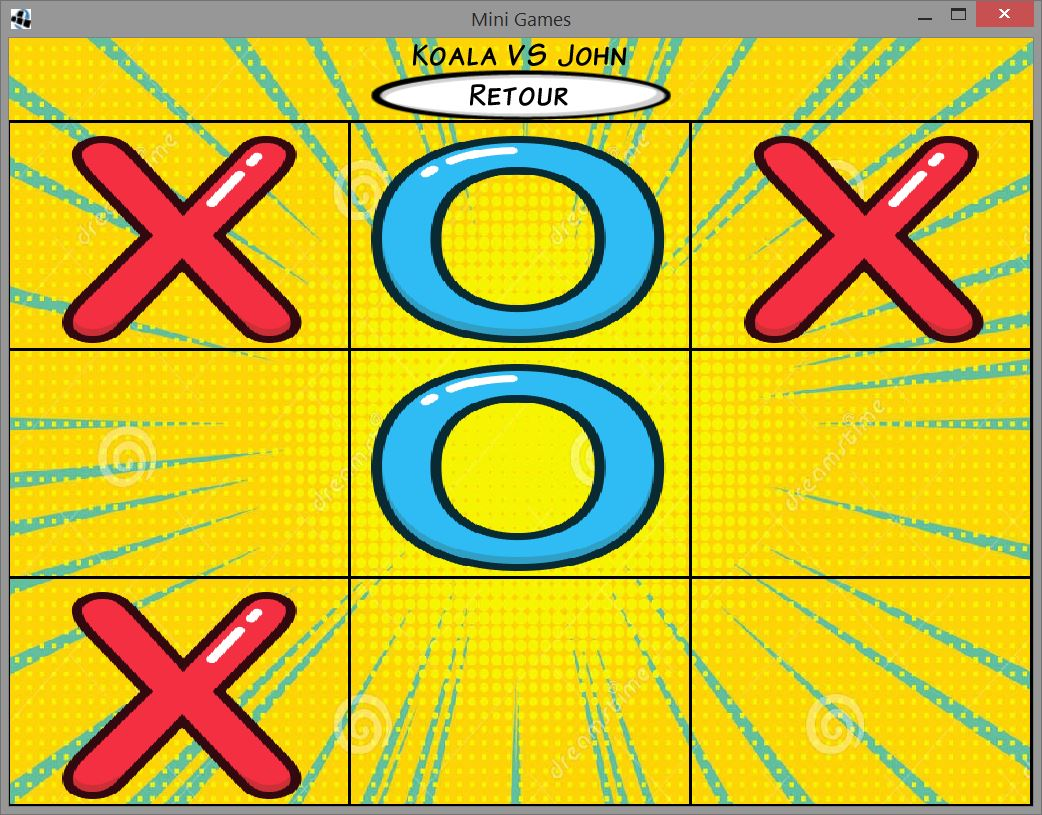
\includegraphics[width=9cm]{morpioningame}
	\caption{Ecran de jeu du morpion}
  \label{morpion_en_jeu}
\end{figure}

Il s'agit du jeu tour par tour, c'est la raison pour laquelle au lancement du jeu un message est envoyé à chaqu'un des joueurs de la parties
leur donnant des indications sur ce qu'ils doivent faire ("c'est votre tour" ou "tour de l'adversaire").
Comme dit plus haut le plateau de jeu est un tabeau de 3x3 cases, il est donc nécaissaire
de savoir dans quelle case le joueur clique avant tout. LibGDX mais à disposition des listeners de clics sur l'écran ce qui signifie qu'il sera possible
de récupérer les coordonées X et Y du clic. Une fois ces coordonnées obtenues on les ananlysent pour savoir quelle est l'index de la case sur laquelle
le joueur à cliqué. Il est à noter que la récupération de l'index de la case cliquée ne se fait que chez le joueur dont c'est le tour de jouer.

Quand la case est cliquée un paquet contenant les informations du plateau de jeu fraîchement modifié est envoyé au serveur. Celui-ci traitera le plateau de jeu
pour savoir si la partie est terminée ou non, en fonction de cette analyse le seveur enverra aux deux joueurs les paquets correspondant (plateau de jeu +
 changement de joueur ou id du gagnant et plateau de jeu).

\section{Bataille navale}
\label{Bataille navale}

\subsection{Description}
Notre jeu de bataille navale, reprend les règles normales du jeu mais avec quelques différence sur le placement et la découverte des bateaux (ennemies ou aliés). Au lieu de pouvoir placer
des bateaux de taille variable (figure \ref{batailleClassique}) comme dans un jeu classique de bataille navale, notre jeu permet de placer un bateau sur une seule et unique case
voir figure \ref{notreBataille}. Il s'agira alors pour notre adversaire de trouver nos bateaux sur la grille.

\begin{figure}[H]
	\centering
\includegraphics[width=9cm]{batailleClassique}
	\caption{Ecran de bataille navale classique}
	\label{batailleClassiqe}
\end{figure}

\subsection{Implémentation}
Comme pour le morpion, dès qu'un joueur commence une partie il est mis dans une file d'attente d'un adversaire (figure \ref{attente_adversaire}).
Une fois un adversaire trouvé, il y a une phase d'initialisation et à ce moment là le joueur va placer ces bateaux. Une fois l'initialisation confirmée,
la partie peut alors commencer et chacun son tour chaque joueur va alors devoir découvrir les bateaux de son adversaires.

\begin{figure}[H]
	\centering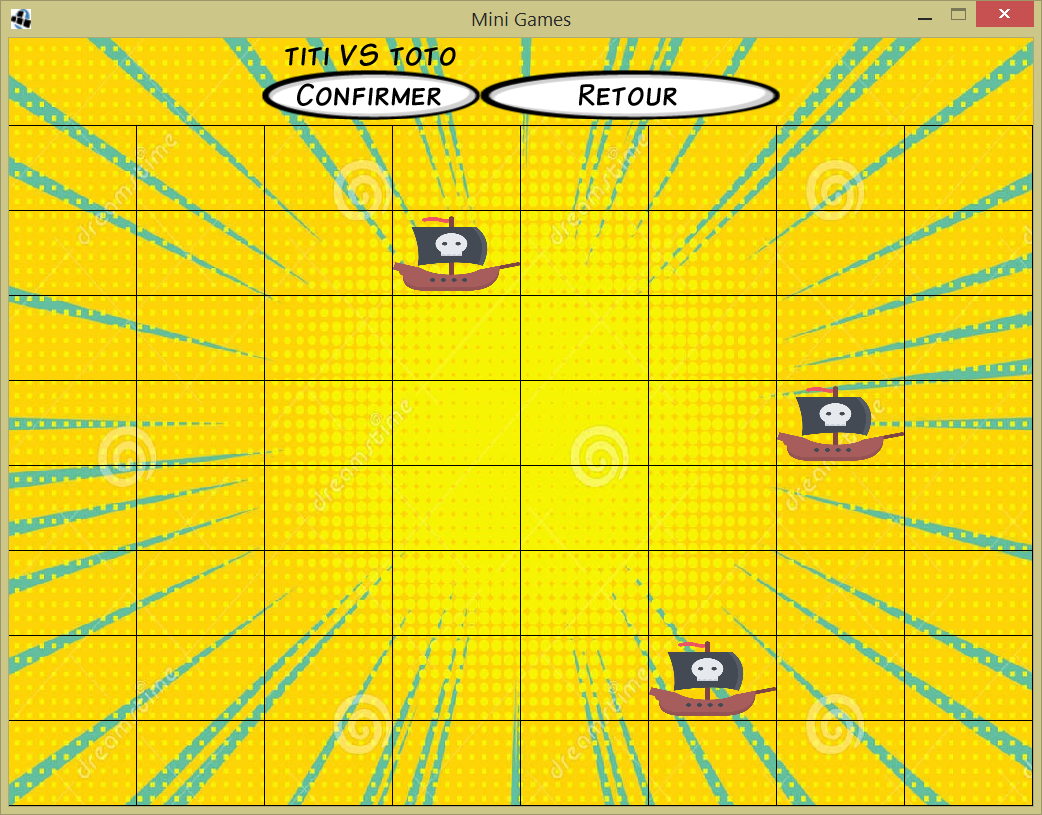
\includegraphics[width=9cm]{notreBataille}
	\caption{Ecran de jeu de la bataille navale}
	\label{notreBataille}
\end{figure}

\chapter{Identité graphique}
Le jeu possède un style fortement inspiré de l'univers des comic book (bande dessinée principalement américaine)
ce choix d'inspiration est principalement lié à l'utilisation d'un très bon thème graphique pour les éléments
d'interface de LigGDX. Le thème nous plaisant nous avons choisi d'associer notre jeu à cet univers en adaptant l'interface, les
textes et les images. C'est de plus un choix qui sort de l'ordinaire car il est plutôt rare de voir des jeux
reprenant ce sytle graphique ce qui est à notre avis un point positif pour notre projet.
\par
Concernant l'image utilisée en backgroud, il s'agit d'une image dont on peut acheter le droit de diffusion ou tous les droits directement sur internet. Comme il s'agit d'un projet qui n'a pas pour objectif (actuellement) d'être déployé, nous n'avons pas effectué l'achat. Si nous décidions l'inverse, il faudrait payer.

\section{Interface}
L'interface du programme est découpé en trois parties principales :

\begin{itemize}
  \item L'écran de login (firgure \ref{Ecran de login})
  \item Le menu de sélection des minis jeux (figure \ref{Ecran de selection})
  \item Le jeu en lui-même (voir figures aux chapitres \ref{Morpion} et \ref{Bataille navale})
\end{itemize}

\begin{figure}[H]
	\centering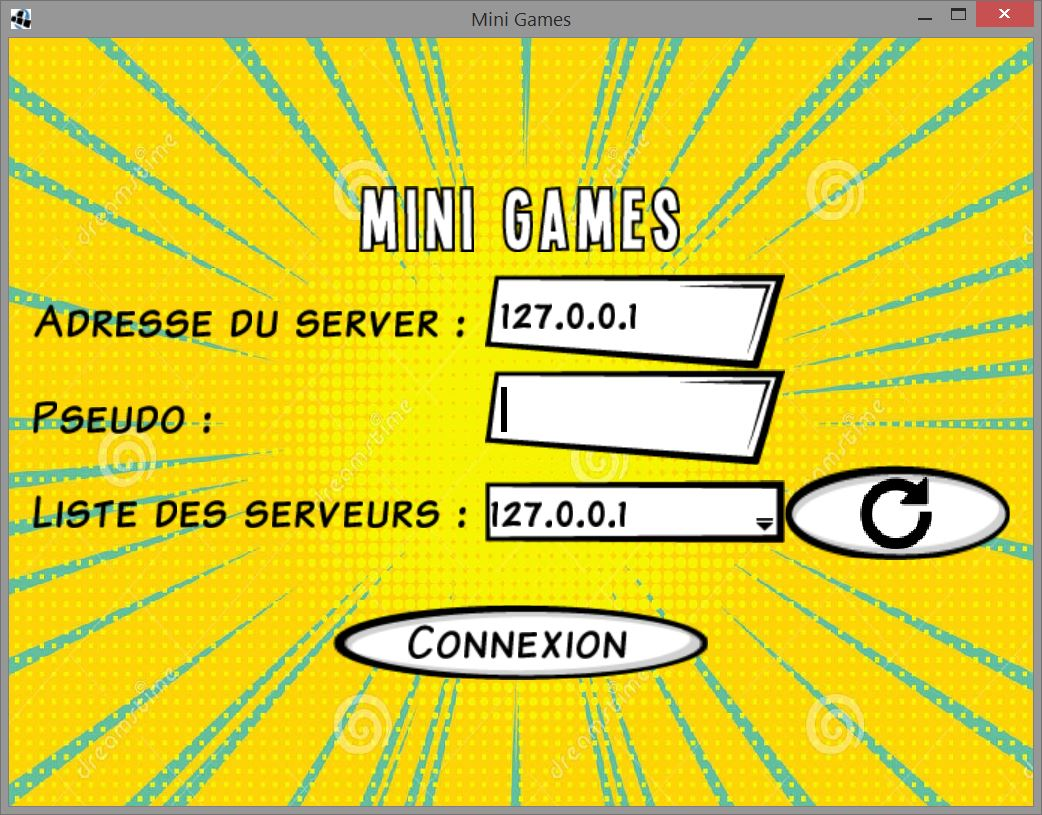
\includegraphics[width=9cm]{loginScreen}
	\caption{Ecran de login}
	\label{Ecran de login}
\end{figure}

\begin{figure}[H]
	\centering\includegraphics[width=9cm]{menuJeux}
	\caption{Ecran de sélection des jeux}
	\label{Ecran de selection}
\end{figure}

LibGDX fournit des objets Table très utile pour organiser des éléments de formulaires sur plusieurs ligne
(à la manière d'un tableau HTML) ils ont été utilisé pour permettre de créer l'aligement de l'écran de login et du menu
présenté ci-dessus.

Les Skins LibGDX sont des collections de ressources graphique utilisés par LibGDX pour personaliser l'ascpect des éléments
de l'interface. LibGDX fournit un skin par défaut mais comme dit dans l'introduction de ce chapitre nous avons opté pour un skin
basé sur le thème des "comics" c'est grâce à lui que nos label,text field,bouton,... ont leur aspect.

\chapter{Tests}
Ce chapitre présente les différents tests qui ont été effectué sur le programme.
\section{Client}
\subsection{Login}
\begin{itemize}
  \item Le programme se lance correctement
  \item L'utilisateur à le focus sur l'entré du pseudo
  \item La touche "Enter" du clavier lance la tentative de connexion
  \item Le bouton "connexion" lance la tentative de connexion
  \item Message d'erreur s'il l'adresse de  serveur n'est pas correcte
  \item Message d'erreur s'il n'y a pas de pseudo
  \item Découvrte des serveur dans le réseau local
  \item Changement de l'adresse du serveur lors de la sélection d'un des éléments de la liste des serveur
  \item Le bouton "refresh" relance la recherche de serveur
  \item Bonne disposition des éléments graphique dans la fenêtre

\end{itemize}

\subsection{Menu des minis jeux}
\begin{itemize}
  \item Affichage du nom du joueur
  \item Bonne disposition des éléments graphique de la fenêtre
  \item Le bouton "retour" renvoie le client à la page de connexion
  \item Le bouton "quitter" quitte le programme
  \item Le bouton "jouer au morpion" lance une partie de morpion
  \item Le bouton "jouer à la bataille navale" lance une partie de bataille navale
\end{itemize}

\subsection{Morpion}
\begin{itemize}
  \item Le joueur est mis en attente s'il est seul à vouloir jouer
  \item Le texte "Attente d'un autre joueur" s'affiche pendant l'attente d'une adversaire
  \item Le bouton "retour" renvoie à au menu de sélection des jeux
  \item La partie se lance quand deux joueurs lance partie sur le même serveur
  \item Un text indique lequel des deux joueurs doit jouer
  \item Si c'est n'est pas le tour du joueur cliquer dans l'air de jeu ne fait rien
  \item Si c'est le tour du joueur cliquer dans l'air de jeu informe le serveur du choix de case
  \item Les joueurs recoivent le plateau de jeu mis à jour par le serveur
  \item Si un joueur a gagne les deux joueurs recoivent des infos du serveur signifiant la fin de la partie
  \item Le text "vous avez gagné" s'affiche chez le gagnant
  \item Le text "vous avez perdu" s'affiche chez le perdant
  \item Le text "égalié" s'affiche en cas d'égalité
  \item Quand la partie est terminé si les joueurs clique sur l'écran ils retourent au menu de sélection des minis jeux
  \item Le text "votre adversaire a quitter la partie" s'affiche si l'adversaire du joueur a quitter la partie
\end{itemize}

\subsection{Bataille navale}


\section{Serveur}

\subsection{Initialisation}
\begin{itemize}
  \item Le serveur se lance correctement
  \item Des clients peuvent se connecter au serveur
  \item le seveur peut recevoir des Packets des clients
  \item le serveur peut envoyer des Packets aux clients
  \item Les joueurs sont sauvegardés dans une liste
  \item Les Games (les jeux) sont sauvegardés dans une liste
\end{itemize}

\subsection{Morpion}
\begin{itemize}
  \item Si personne n'est en attente sur ce jeu le joueur est mis en attente
  \item Si un joueur est déjà en attente une partie est lancée
  \item Si un joueur quitte la partie quand il est en attente il n'est plus en attente
  \item Le serveur reçoit des Packets donnant des informations sur le plateau de jeu de la part des joueurs
  \item Le serveur test si la partie est gagnée ou non
  \item Le serveur renvoie de nouvelle infos sur la partie aux deux joueurs
  \item Si un joueur se déconnecte ou s'il appuie sur le bouton retoure le serveur est notifié
  \item Le serveur envoie un Packet à au joueur dont l'adversaire a quitter la partie
\end{itemize}

\subsection{Bataille navale}





\chapter{Problematique}
Une des problématique rencontrée a été la mise en place d'un serveur sur android. En effet, LibGDX "facile" le portage de l'application client vers les
périphériques android mais le serveur à lui été dévelopé sans libgdx. Une ébauche d'application android oppérant de la même manière que le serveur Java classique a
été mise en place, l'implémentation c'est avérée très lourdes et peu fructueuse dans le sens où lorsqu'un client se connectait à un serveur android celui-ci crashait
immédiatement.

Dans de très rares cas il est également possible que le lancement de la partie ne s'effectue pas tout à fait correctement. Une des deux joueurs aura déjà l'écran du début de partie alors
que l'autre affiche toujours l'écran d'attente. Cela c'est cependant pas un problème majeur car si ce problème survient les deux joueurs on accès à un bouton "retour" leur
permettant de revenir à la sélection des minis jeux et de relancer une partie.

Un autre problème que nous avons rencontré est le fait que, pour des raisons de performences, LibGDX n'est pas thread-safe, ce qui fait que, en fonction de l'ordre d'arrivée des paquets, il est possible que le programme tente d'accéder à une ressource qui n'existe pas encore. Il s'agit d'un problème connu de LibGDX qui, pour l'instant, refuse de le corriger afin de garder leurs performences. Cependant, ce problème n'arrivant que lors de très rares occasions, il aurait été trop couteux en terme de ressources de le corriger et s'assurer que le fix était bien effectif car nous n'avons pas moyen de trouver quel appel devrait être exécuté sans changement de contexte (atomique).

Le programme requiert également une grande quantité de mémoire ce qui nous laisse penser que tous n'est pas supprimé comme il devrait l'être.

\chapter{Améliorations}
La communication entre pc et android est fonctionnelle mais, comme expliqué plus haut, notre shouaite était d'étendre notre proramme à encore deux autres
plate-formes : IOS et HTML5 (navigateur web). Certain problème d'implpémentation pourrait survenir (utilisation d'outil non supportés sur certaines plate-formes, etc.)
mais avec du temps l'application pourrait être totalement multi-plateforme.
De nouveaux jeux pourraient aussi être rajoutés tels que ,comme décrit dans notre cahier des charges comme objectif bonus,
un jeu de dame ou encore bien d'autre jeux. Un système de point pourrait être attribuer les joueus les récompansant d'avoir gagnés une
partie par exmple. Les points pourraient être utilisés pour mettre en place un classement des meilleurs joueurs du serveur.

\chapter{Conclusion}
Nous avons pu réaliser les objectifs primaire que nous nous étions fixés dans le cahier des charges, nous
sommes donc satisfait du résultat. Une de nos plus grosses attente était de pouvoir continuer d'apprendre à
utiliser des outils tel que LibGDX ou Kryonet et nous avons été agréblement surpis de la faciliter de mise
en place de ces deux outils dans un même environnement.

\chapter{Bibliographie}

\href{http://www.flaticon.com/free-icon/pirate-ship_361245#term=pirate%20ship&page=1&position=6}{Lien de l'image du bateau pirate}

\href{https://www.dreamstime.com/stock-illustration-retro-comic-background-old-yellow-green-halftone-gradient-pop-art-style-image81648431}{Lien de l'image du background}


https://github.com/libgdx/libgdx/issues/3491

\end{document}
